\documentclass[10pt,twocolumn,letterpaper]{article}
\usepackage{ctex}
\usepackage{CJK}
\usepackage{graphicx}
\usepackage{booktabs}
\usepackage[justification=centering]{caption}
\bibliographystyle{abbrv}
\setlength{\parindent}{2em}
\begin{document}
\title{Optical systems}
\author{Qilei Zhang}
\date{may 27 2018}
\maketitle
\section{introduction}
  Stochastic resonance was realized in an electronic circuit,a simple Schmitt trigger (Fauve and Heslot, 1983). Since then, stochastic resonance has been observed in a variety of more or less complicated electronic devices, mostly constructed with the purpose of building flexible and inexpensive simulation tools.
\begin{figure}[htbp]
\small
\centering
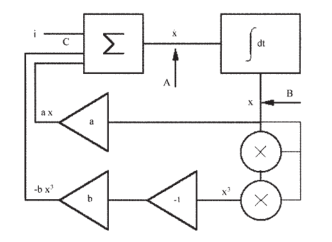
\includegraphics[width=20em]{023.png}
\caption{23 Bistable ring laser}
\label{fig:lable}
\end{figure}
\section{Analog electronic simulators}
As mentioned in Sec. II.C, electronic circuits have been widely employed in the study of nonlinear stochastic equations.\cite{Alpher02} The realization of an electronic simulation circuit requires the design of specific electronic devices which operate as the single components of the block scheme depicted in Fig. 23.
\begin{equation}
\quad x'=x-x^3+u(t)+A_0 cos(st)
\end{equation}
\section{Electron paramagnetic resonance}
An EPR system consists of a paramagnetic sample placed in a microwave cavity. A microwave generator irradiates the sample while a feedback electronic circuit locks the oscillator frequency to the resonant frequency Nc of the cavity.\cite{Alpher04}\\


\section{Superconducting quantum interference devices}
The basic components of a SQUID are a superconducting loop and a Josephson junction. For practical purposes, a SQUID can be envisioned as an electromagnetic device that converts a magnetic flux variation into a voltage variation and, as such, it has been successfully employed in monitoring small magnetic field fluctuations.\cite{Alpher03}\\
\begin{table}
\begin{center}
\begin{tabular}{cccccccc}
\toprule
         & 1 &  2  &   3  &  4  &  5  &  6  & 7 \\
\midrule
Alphabet & A &  B  &   C  &  D  &  E  &  F  & G\\
Roman    & I &  II &  III &  IV &  V  &  VI & VII\\
\bottomrule
\end{tabular}
\end{center}
\caption{Results.   Ours is better.}
\end{table}
\bibliography{zzz}
\end{document}

